\documentclass[journal,12pt,twocolumn]{IEEEtran}

\usepackage{setspace}
\usepackage{gensymb}
\singlespacing
\usepackage[cmex10]{amsmath}

\usepackage{amsthm}

\usepackage{mathrsfs}
\usepackage{txfonts}
\usepackage{stfloats}
\usepackage{bm}
\usepackage{cite}
\usepackage{cases}
\usepackage{subfig}

\usepackage{longtable}
\usepackage{multirow}

\usepackage{enumitem}
\usepackage{mathtools}
\usepackage{steinmetz}
\usepackage{tikz}
\usepackage{circuitikz}
\usepackage{verbatim}
\usepackage{tfrupee}
\usepackage[breaklinks=true]{hyperref}
\usepackage{graphicx}
\usepackage{tkz-euclide}


\usetikzlibrary{calc,math}
\usepackage{listings}
    \usepackage{color}                                            %%
    \usepackage{array}                                            %%
    \usepackage{longtable}                                        %%
    \usepackage{calc}                                             %%
    \usepackage{multirow}                                         %%
    \usepackage{hhline}                                           %%
    \usepackage{ifthen}                                           %%
    \usepackage{lscape}     
\usepackage{multicol}
\usepackage{chngcntr}

\DeclareMathOperator*{\Res}{Res}

\renewcommand\thesection{\arabic{section}}
\renewcommand\thesubsection{\thesection.\arabic{subsection}}
\renewcommand\thesubsubsection{\thesubsection.\arabic{subsubsection}}

\renewcommand\thesectiondis{\arabic{section}}
\renewcommand\thesubsectiondis{\thesectiondis.\arabic{subsection}}
\renewcommand\thesubsubsectiondis{\thesubsectiondis.\arabic{subsubsection}}


\hyphenation{op-tical net-works semi-conduc-tor}
\def\inputGnumericTable{}                                 %%

\lstset{
%language=C,
frame=single, 
breaklines=true,
columns=fullflexible
}
\begin{document}


\newtheorem{theorem}{Theorem}[section]
\newtheorem{problem}{Problem}
\newtheorem{proposition}{Proposition}[section]
\newtheorem{lemma}{Lemma}[section]
\newtheorem{corollary}[theorem]{Corollary}
\newtheorem{example}{Example}[section]
\newtheorem{definition}[problem]{Definition}

\newcommand{\BEQA}{\begin{eqnarray}}
\newcommand{\EEQA}{\end{eqnarray}}
\newcommand{\define}{\stackrel{\triangle}{=}}
\bibliographystyle{IEEEtran}
\raggedbottom
\setlength{\parindent}{0pt}
\providecommand{\mbf}{\mathbf}
\providecommand{\pr}[1]{\ensuremath{\Pr\left(#1\right)}}
\providecommand{\qfunc}[1]{\ensuremath{Q\left(#1\right)}}
\providecommand{\sbrak}[1]{\ensuremath{{}\left[#1\right]}}
\providecommand{\lsbrak}[1]{\ensuremath{{}\left[#1\right.}}
\providecommand{\rsbrak}[1]{\ensuremath{{}\left.#1\right]}}
\providecommand{\brak}[1]{\ensuremath{\left(#1\right)}}
\providecommand{\lbrak}[1]{\ensuremath{\left(#1\right.}}
\providecommand{\rbrak}[1]{\ensuremath{\left.#1\right)}}
\providecommand{\cbrak}[1]{\ensuremath{\left\{#1\right\}}}
\providecommand{\lcbrak}[1]{\ensuremath{\left\{#1\right.}}
\providecommand{\rcbrak}[1]{\ensuremath{\left.#1\right\}}}
\theoremstyle{remark}
\newtheorem{rem}{Remark}
\newcommand{\sgn}{\mathop{\mathrm{sgn}}}
\providecommand{\abs}[1]{\ensuremath{\left \vert #1\right\vert}}
\providecommand{\res}[1]{\Res\displaylimits_{#1}} 
%\providecommand{\norm}[1]{\left\lVert#1\right\rVert}
%\providecommand{\norm}[1]{\lVert#1\rVert}
\providecommand{\mtx}[1]{\mathbf{#1}}
%\providecommand{\mean}[1]{E\left[ #1 \right]}
\providecommand{\fourier}{\overset{\mathcal{F}}{ \rightleftharpoons}}
%\providecommand{\hilbert}{\overset{\mathcal{H}}{ \rightleftharpoons}}
\providecommand{\system}{\overset{\mathcal{H}}{ \longleftrightarrow}}
	%\newcommand{\solution}[2]{\textbf{Solution:}{#1}}
\newcommand{\solution}{\noindent \textbf{Solution: }}
\newcommand{\cosec}{\,\text{cosec}\,}
\providecommand{\dec}[2]{\ensuremath{\overset{#1}{\underset{#2}{\gtrless}}}}
\newcommand{\myvec}[1]{\ensuremath{\begin{pmatrix}#1\end{pmatrix}}}
\newcommand{\mydet}[1]{\ensuremath{\begin{vmatrix}#1\end{vmatrix}}}
\numberwithin{equation}{subsection}
\makeatletter
\@addtoreset{figure}{problem}
\makeatother
\let\StandardTheFigure\thefigure
\let\vec\mathbf
\renewcommand{\thefigure}{\theproblem}
\def\putbox#1#2#3{\makebox[0in][l]{\makebox[#1][l]{}\raisebox{\baselineskip}[0in][0in]{\raisebox{#2}[0in][0in]{#3}}}}
     \def\rightbox#1{\makebox[0in][r]{#1}}
     \def\centbox#1{\makebox[0in]{#1}}
     \def\topbox#1{\raisebox{-\baselineskip}[0in][0in]{#1}}
     \def\midbox#1{\raisebox{-0.5\baselineskip}[0in][0in]{#1}}
\vspace{3cm}
\title{AI1103 ASSIGNMENT 4}
\author{Name:MANNAM SARANDEEP,Rollno:CS20BTECH11030}
\maketitle
\newpage
\bigskip
\renewcommand{\thefigure}{\theenumi}
\renewcommand{\thetable}{\theenumi}
\newcommand{\dsum}{\displaystyle\sum}
\newcommand{\R}{\mathbb{R}}
\newcommand{\C}{\mathbb{C}}


Download the python code from 
\begin{lstlisting}
https://github.com/sarandeepmannam/ASSIGNMENT4/blob/main/Assignment4.py
\end{lstlisting}
%
and latex-tikz code from 
%
\begin{lstlisting}
https://github.com/sarandeepmannam/ASSIGNMENT4/blob/main/Assignment4.tex
\end{lstlisting}
\section{Question-CSIR UGC NET June 2012,Q.50}
Let $X_{1},X_{2},....$ be i.i.d N(1,1) random variables.Let $S_{n}=X_{1}^{2}+X_{2}^2+...+X_{n}^{2}$ for $n\ge1$.Then $$\lim_{n \to \infty}{\frac{Var\brak{S_{n}}}{n}}=$$
\begin{enumerate}[label = (\Alph*)]
\item  $4$
\item  $6$
\item  $1$
\item  $0$
\end{enumerate}

\section{Solution-CSIR UGC NET June 2012,Q.50}

\begin{definition}[NON-CENTRAL CHI SQUARE DISTRIBUTION]
Let $X_{1},X_{2},X_{3}.,X_{i},.X_{n}$ be n independent, normally distributed random variables with means $\mu_{i}$ and unit variances.Then the random variable
$$\sum_{i=0}^{n}X_{i}$$ is distributed according to the non-central chi square distribution.It has two parameters 'k' which specifies the number of degrees of freedom (i.e. the number of $X_{i}$), and '$\lambda$' which is called non-centrality parameter given by,
\begin{align}
    \lambda=\sum_{i=0}^{n}\mu_{i}^2
\end{align}
\label{def-NCSD}
\end{definition}
From definition \ref{def-NCSD},
Since $X_{1},X_{2},...$ are i.i.d N(1,1) normal random variables therefore the distribution of the random variable $S_{n}=X_{1}^{2}+X_{2}^{2}+...X_{n}^{2}$ is a non-central chi square distribution with 'n' degrees of freedom and non-centrality parameter '$\lambda$' given by
\begin{align}
    \lambda&=\sum_{i=1}^{n}(\mu_{i})^{2}
    \\\lambda&=\sum_{i=1}^{n}1=n
    \end{align}
\begin{lemma}
Moment generating function of a non-central chi square distributed random variable X is given by,
\begin{align}
    M_{X}(t)=\frac{e^{\frac{\lambda t}{1-2t}}}{(1-2t)^{\frac{n}{2}}}
\end{align}
\label{MGF}
\end{lemma}


From Lemma \ref{MGF} Moment generating function of $S_{n}$ is given by,
\begin{align}
    M_{S_{n}}(t)&=\frac{e^{\frac{n t}{1-2t}}}{(1-2t)^{\frac{n}{2}}}
\end{align}


\begin{figure}[h]
 \centering
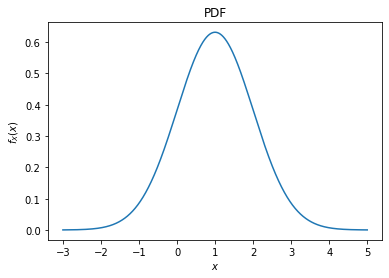
\includegraphics[width=\columnwidth]{PDF.png}
 \caption{PDF of $X_{1},X_{2},..$}
    \label{fig:my_label}
\end{figure}

\newpage

\begin{definition}[nth moment]
 The nth moment of a random variable $X$ about a number $k$ is the expected value of the nth power of the deviations of $X$ about $k$ and is given by $E((X-k)^{n})$.
 
 \label{nth-mom}
\end{definition}
From definition \ref{nth-mom},the nth moment of a random variable $X$ about $0$ is given by $E(X^{n})$, which is the expected value of nth power of $X$.
\begin{lemma}
 The nth moment of a random variable $X$ about $0$ whose MGF is $M_{X}(t)\brak{\equiv E(e^{tX})}$ is the value of the nth derivative of the MGF at $0$ and is given by,
 \begin{align}
     E(X^{n})=\brak{\frac{d^{n}}{dt^{n}}\brak{M_{X}(t)}}_{t=0}
     \label{4}
 \end{align}
 \label{Moment}
\end{lemma}
\begin{proof}
\begin{align}
    M_{X}(t)\equiv E(e^{tX})
\end{align}
Using taylor series,
\begin{align}
e^{tX}&=1+\frac{tX}{1!}+\frac{(tX)^2}{2!}+\frac{(tX)^3}{3!}+..+\frac{(tX)^n}{n!}+..
\end{align}
Therefore,
\begin{align}
 M_{X}(t)&=E(1+\frac{tX}{1!}+\frac{(tX)^2}{2!}+\frac{(tX)^3}{3!}+..+\frac{(tX)^n}{n!}+..)
 \\M_{X}(t)&=E(1)+tE\brak{\frac{X}{1!}}+t^{2}E\brak{\frac{X^2}{2!}}+t^3E\brak{\frac{X^3}{3!}}+...
\end{align}
Taking $n$th derivative  on both sides with respect to '$t$' at $t=0$ we get,
\begin{multline}
\brak{\frac{d^{n}}{dt^{n}}\brak{M_{X}(t)}}_{t=0}=\brak{E(X^n)}_{t=0}+\brak{tE\brak{\frac{X^{n+1}}{n+1}}}_{t=0}\\
+\brak{t^2E\brak{\frac{X^{n+2}}{(n+1)(n+2)}}}_{t=0}+...
\end{multline}
\begin{align}
    \brak{\frac{d^{n}}{dt^{n}}\brak{M_{X}(t)}}_{t=0}=E(X^{n})
\end{align}
\end{proof}
From lemma \ref{Moment} ,
\begin{align}
 E(S_{n})&=\brak{\frac{d}{dt}\brak{M_{S_{n}}(t)}}_{t=0}
\\E(S_{n})&=\brak{\frac{2ne^{\frac{nt}{1-2t}}}{(1-2t)^{\frac{n}{2}+2}}(1-t)}_{t=0}
\\\implies  E(S_{n})&=2n \label{2}
\end{align}
From lemma \ref{Moment},
\begin{align}
  E(S_{n}^2)=\brak{\frac{d^{2}}{dt^{2}}\brak{M_{S_{n}}(t)}}_{t=0}
\end{align}
\begin{multline}
 E(S_{n}^2)=\frac{2ne^{\frac{nt}{1-2t}}}{(1-2t)^{\frac{n}{2}+4}}(n(1-t)-(1-2t)^{2}\\
 +(1-t)(1-2t)(n+4))|_{t=0}
\end{multline}
\begin{align}
E(S_{n}^2)&=\frac{2n}{1^{n/2+2}}\brak{n-1^2+n+4}
\\E(S_{n}^2)&=2n\times(2n+3)
\\\implies E(S_{n}^2)&=4n^{2}+6n
\label{3}
\end{align}

Variance of $S_{n}$,
\begin{align}
Var(S_{n})&=E(S_{n}^2)-(E(S_{n}))^2
\label{1}
\end{align}
Substituting equations (\ref{2}) and (\ref{3}) in (\ref{1}),we get 
\begin{align}
    Var(S_{n})&=4n^{2}+6n-\brak{2n}^{2}
\\ \implies Var(S_{n})&=6n
\end{align}
and
$$\lim_{n \to \infty}{\frac{Var\brak{S_{n}}}{n}}=\lim_{n \to \infty}{\frac{6n}{n}}=\lim_{n \to \infty}{6}=6$$

Hence,option(B) is correct.
    
 
\end{document}
